
%!TEX root = ../terrainbook.tex

\graphicspath{{kriging/}}

\chapter{Spatial interpolation: kriging}
\label{chap:kriging}


Kriging is a spatial interpolation method that was developed mostly by Georges Matheron based on the earlier work of Danie Krige, who used it to estimate the gold yields of mines in South Africa.
In contrast to the other spatial interpolation methods seen in \refchap{chap:interpol}, it uses a statistical model to take into account the varying uncertainty and spatial correlation of a set of sample points.

Kriging is based on the fact that when one moves across space, values such as the gold content in rock and the elevation in a terrain have both a certain spatial trend (\eg\ a mean value, a fitted plane or a more complex polynomial) and also a certain spatially correlated randomness (\ie\ closer points tend to have more similar values).

In the simplest cases, when the trend is completely known, it is possible to use \emph{simple kriging}, which is rather uncommon in practice and thus not covered in this course.
Instead, we will look at the simplest case that is common in practice: \emph{ordinary kriging}.

\section{Basic concepts}

The physical processes that shape the world are often considered to be deterministic.
In the case of a DTM, the elevation is determined by well-known processes that we can model, such as plate tectonics, volcanic activity and erosion.
However, these processes are so complex that elevation values appear to be generated at least partly randomly.
In geostatistics, the value of properties such as the elevation are thus defined as the result of \emph{random processes}.

Because of this inherent randomness, geostatistics considers that the sampled value of a property at a location \(x\) is just one of the infinitely many values that are possible at that location.
These possible values are represented by a \emph{probability distribution}, which we can associate with standard statistical measures, such as the mean and variance.
This situation is modelled mathematically by saying that the value of the property at \(x\) is a \emph{random variable} \(Z\).

The statistical concept of the mean is equivalent to the \emph{expectation}, or \emph{expected value}, of a random variable, which is denoted as \(E[Z]\).
Based on this definition, it is possible to then define the \emph{variance} of a random variable \(Z\), which is denoted as \(\mathrm{var}(Z)\) or \(\sigma^2\) and is a measure of how far the values of \(Z\) will usually spread from its mean.
Mathematically, it is defined as the expected value of the squared deviation from the expected value of \(Z\), or:

\begin{equation}
\mathrm{var}(Z) = E\left[{\left(Z-E\left[Z\right]\right)}^2\right] = E[Z^2]-{(E[Z])}^2.
\end{equation}

Next, it is important to define the covariance, denoted as \(\mathrm{cov}(Z_i,Z_j)\), or \(\sigma_{ij}\), which expresses the joint variability of two random variables.
Thus, a positive covariance between \(Z_i\) and \(Z_j\) means that when one increases or decreases, the other is expected to increase/decrease in the same direction.
Conversely, a negative covariance means that the variables tend to increase/decrease in opposite directions.
The magnitude of the covariance is related to the magnitude of this increase or decrease.
It is thus defined mathematically as the expected product of their deviations from their (individual) expected values, or:

\begin{equation}
\mathrm{cov}(Z_i,Z_j) = E\left[\left(Z_i-E[Z_i]\right)\left(Z_j-E[Z_j]\right)\right].
\end{equation}

Note that the covariance of \(Z_i\) with itself is equivalent to the variance of \(Z_i\):

\begin{equation}
\mathrm{cov}(Z_i,Z_i) = E\left[\left(Z_i-E[Z_i]\right)^2\right] = \mathrm{var}(Z_i).
\end{equation}

While not used further in this chapter, it is good to know that the variance and the covariance can be used to calculate the Pearson correlation coefficient \(\rho_{ij}\), which is the most common correlation coefficient:

\begin{equation}
\rho_{ij}=\frac{\mathrm{cov}(Z_i, Z_j)}{\sqrt{\mathrm{var}(Z_i) \mathrm{var}(Z_j)}}.
\end{equation}

Note that this is essentially just a normalised form of the covariance.

\section{The variogram}

The previous equations for the variance and the covariance are \emph{theoretical} and do not directly account for the uncertainty and the spatial correlation of the sample points.
In order to estimate the covariance that takes these factors into account experimentally, kriging thus generally relies on what is known as a \emph{variogram}.
The variogram \(\gamma(h)\) is a function that expresses the average dissimilarity of the value of a random variable \(Z\) between sample points at different distances.
It is defined as:

\begin{equation}
\gamma(h) = \frac{1}{2} (Z(x+h) - Z(x))^2,
\end{equation}

where \(x\) is a sample point, \(h\) is a vector from \(x\) to another sample point and \(Z(x)\) is the value of a random variable at \(x\) (\eg\ its elevation).

When this is done with every possible pair of sample points in a dataset, or with a representative subset in order to speed up the process as it is usually done in practice, \(|h|\) (\ie\ the magnitude of the vector \(h\)) and \(\gamma(h)\) can be put into a scatter plot to show how the average dissimilarity of a value changes with the distance between the sample points.
The result of such a plot is what is known as a \emph{variogram cloud} (Figure~\ref{fig:variogram_cloud}).

\begin{figure}[htbp]
\begin{subfigure}{0.5\linewidth}
\centering
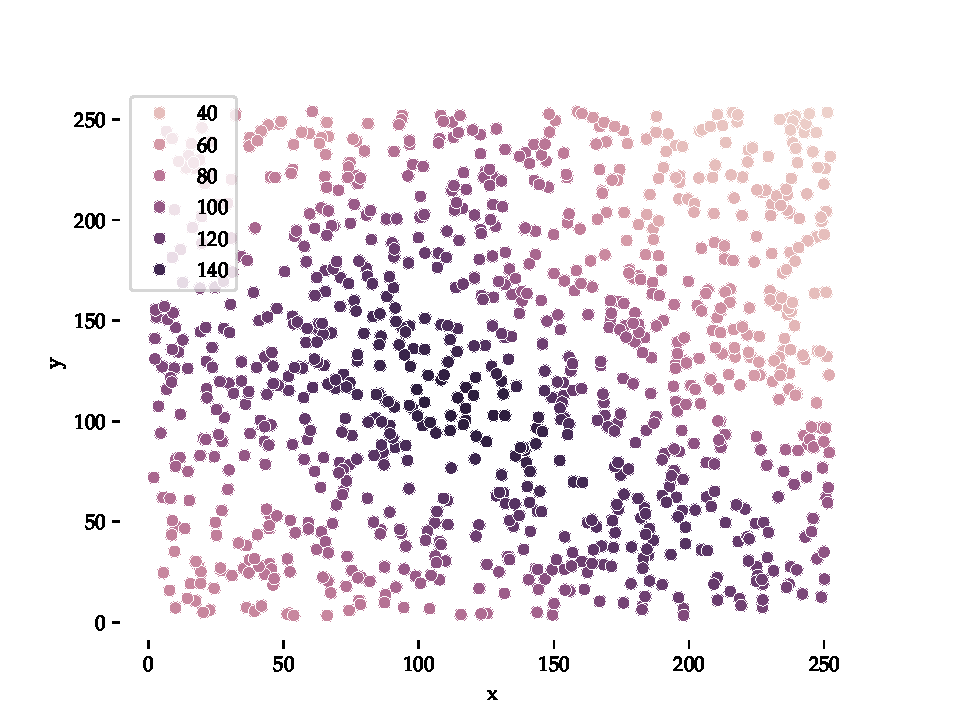
\includegraphics[width=\linewidth]{figs/data}
\caption{dataset}
\end{subfigure}%
\begin{subfigure}{0.5\linewidth}
\centering
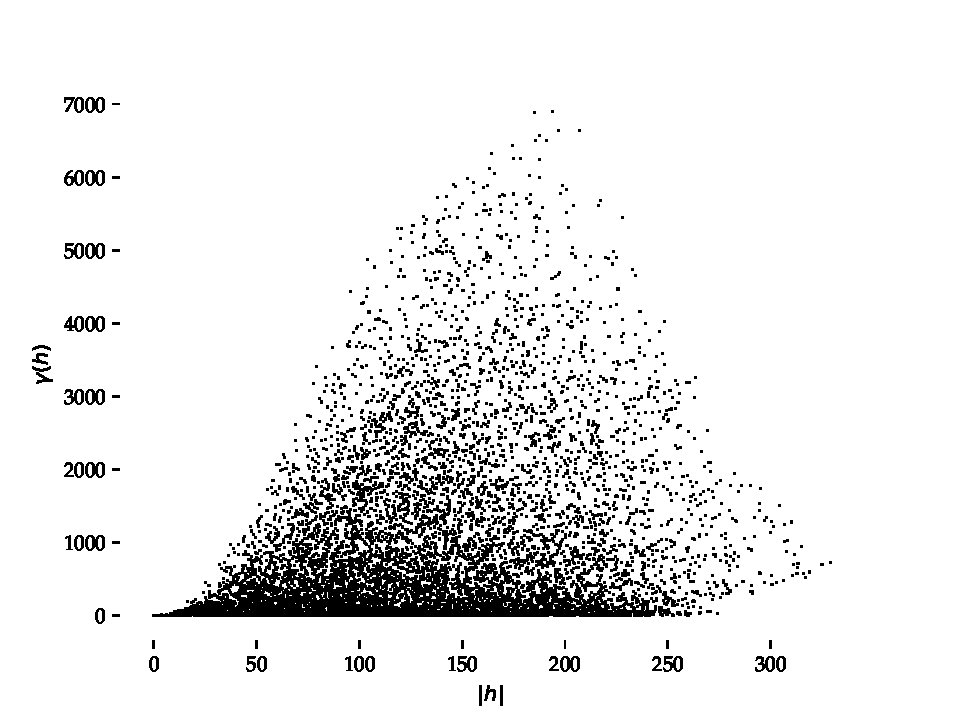
\includegraphics[width=\linewidth]{figs/variogram_cloud}
\caption{variogram cloud}
\end{subfigure}%
\caption{Starting from (a) a sample dataset, (b) the variogram cloud can be computed.
In this case, only 1\% randomly selected point pairs were used.}%
\label{fig:variogram_cloud}
\end{figure}

In this figure, it is possible to see some typical characteristics of a variogram cloud.
Since nearby sample points tend to have similar values, the dissimilarity tends to increase as the distance between sample points increases.
However, it is worth noting that since the farthest away pairs of sample points have similar values in this dataset, the dissimilarity also decreases at the highest distances.

Since most of the time there is a wide variation between the dissimilarities shown at all distances in a variogram cloud, the next step is to average the dissimilarity of the pairs of sample points based on distance intervals.
Mathematically, a series of averages of dissimilarities \(\gamma^\star(h)\) can be created by computing the average dissimilarities for all vectors whose lengths are within a series of specified intervals (generally known as \emph{bins}).
Given a set \(\mathfrak{h}\) containing the vectors for a length interval, the average for its dissimilarity class is computed as:

\begin{equation}
\gamma^\star(\mathfrak{h}) = \frac{1}{2n}\sum\left(z\left(x+h\right)-z\left(x\right)\right)^2 \hspace{1cm}\text{for all } h \in \mathfrak{h}
\end{equation}

where \(n\) is the number of sample point pairs in \(\mathfrak{h}\).

This computation results in much smoother values for the dissimilarity, and when the results of \(|h|\) and \(\gamma^\star(h)\) are put into a scatter plot (Figure~\ref{fig:experimental_variogram}), the result is what is known as an \emph{experimental variogram}.
Experimental variograms are based on a few parameters (Figure~\ref{fig:experimental_variogram}b illustrates these): 
\begin{itemize}
  \item the \emph{sill}, which is the upper bound of \(\gamma^\star(h)\); 
  \item the \emph{range}, which is the value of \(|h|\) when it converges; 
  \item the \emph{nugget}, which is the value of \(\gamma^\star(h)\) when \(|h| = 0\).
\end{itemize}
Note that in order to avoid the unreliable dissimilarities that are common at large distances between sample points, it is usual practice to only compute the experimental variogram for distances up to half of the size of the region covered by the dataset.

\begin{figure}[htbp]
\begin{subfigure}{0.5\linewidth}
\centering
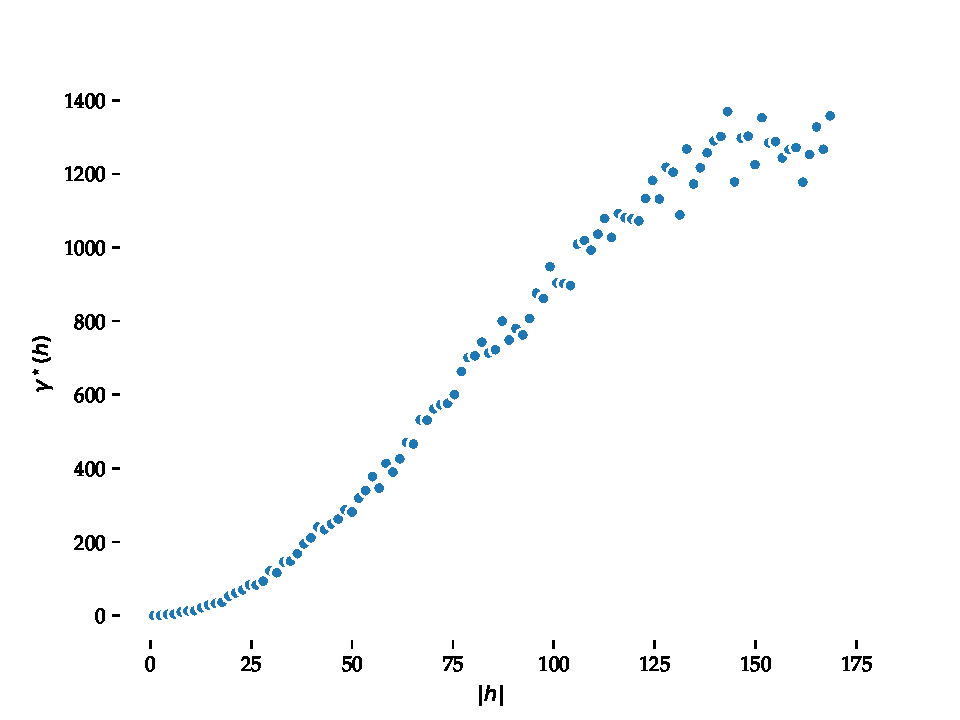
\includegraphics[width=\linewidth]{figs/experimental_variogram}
\caption{experimental variogram}
\end{subfigure}%
\begin{subfigure}{0.5\linewidth}
\centering
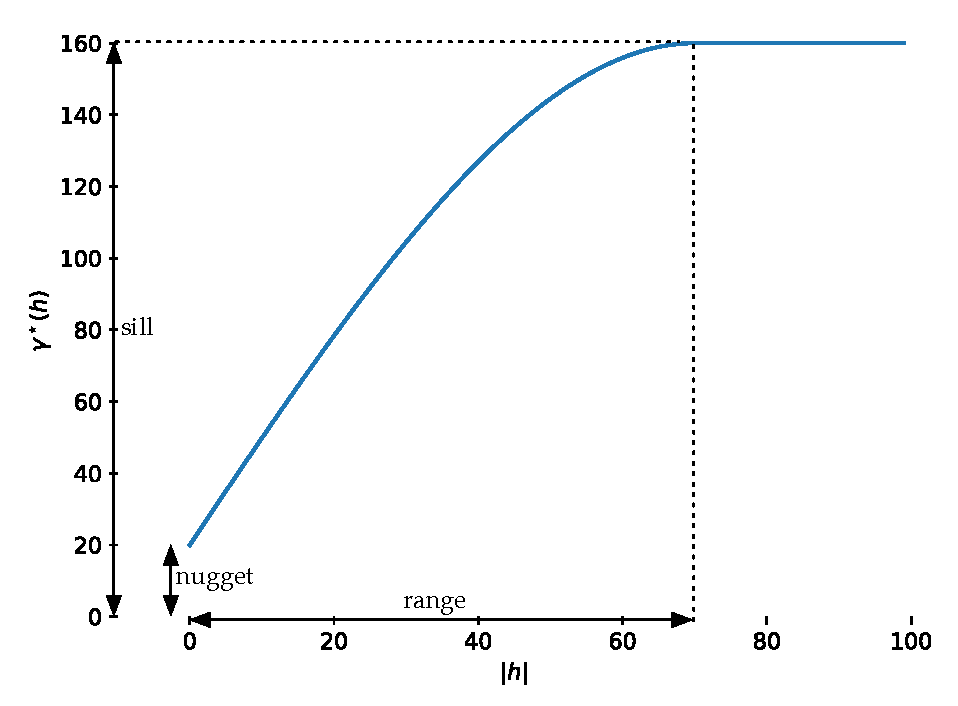
\includegraphics[width=\linewidth]{figs/example_variogram}
\caption{parameters}
\end{subfigure}%
\caption{(a) The experimental variogram is usually described in terms of (b) its parameters.}%
\label{fig:experimental_variogram}
\end{figure}

Finally, the last step is to replace the experimental variogram with a \emph{theoretical variogram} function that approximates it and which can be more easily evaluated for further calculations.
Depending on the shape of the variogram, there are various functions that can be used.
Some examples are:

\begin{align}
\gamma_\mathrm{exponential}(h) &= s \left(1 - e^\frac{-3|h|}{r}\right) + n \\
\gamma_\mathrm{gaussian}(h) &= s \left(1 - e^\frac{-\left(3|h|\right)^2}{r^2}\right) + n \\
\gamma_\mathrm{spherical}(h) &= \begin{cases} 
   s \left(\frac{3|h|}{2r} - \frac{|h|^3}{2r^3}\right) + n & \text{if } |h| \leq r \\
   s + n & \text{if } |h| > r
  \end{cases}
\end{align}

where \(s\) is the \emph{sill}, set to roughly the value of \(\gamma^\star(h)\) when \(\gamma^\star(h)\) is  flat; \(r\) is the \emph{range}, roughly the minimum value of \(|h|\) where \(\gamma^\star(h)\) is flat, and \(n\) is the nugget, which is the starting value of \(\gamma^\star(h)\).
Figure~\ref{fig:theoretical_variogram} shows the result of fitting the three example theoretical variogram functions, exponential, gaussian and spherical.
Note how the gaussian function appears to be a better fit in this case.

\begin{figure}[htbp]
\centering
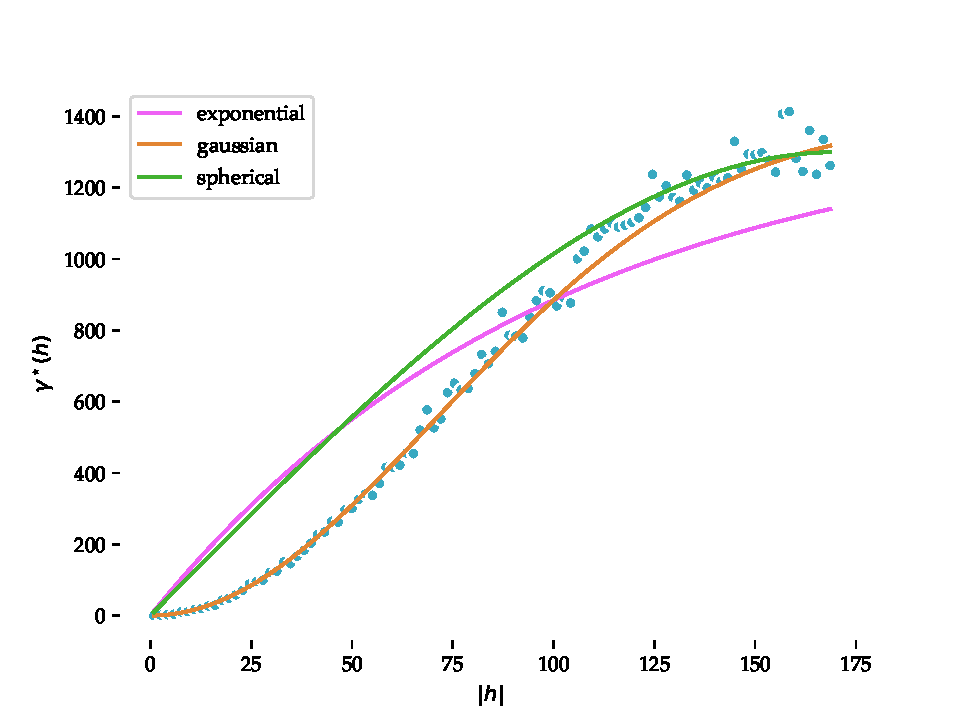
\includegraphics[width=0.5\linewidth]{figs/theoretical_variogram}
\caption{Three possible theoretical variogram functions}%
\label{fig:theoretical_variogram}
\end{figure}

% \section{Linear regression or simple kriging}

\section{Ordinary kriging}

Ordinary kriging is similar to the other spatial interpolation methods that use a weighted average and were described in \refchap{chap:interpol}.
It defines a function \(\hat{Z}\) that estimates the value of the random variable \(Z\) at a location \(x_0\) as a weighted average of its value at the \(n\) sample points \(x_i\) for \(1 \leq i \leq n\) that we will use for the interpolation.
We denote this as:

\begin{equation}
\hat{Z}(x_0) = \sum_{i=1}^n w_i Z(x_i).
\end{equation}

Ordinary kriging has two distinguishing characteristics. First, it is \emph{unbiased}.
This means that it creates a model where the expectation of the estimation is equal to the estimation of the value.
That is, \(E\left[ \hat{Z}(x_0) - Z(x_0) \right] = 0\).
In order to achieve this, the weights should add up to 1.0:

\begin{equation}
\sum_{i=1}^n w_i = 1.
\end{equation}

Second, ordinary kriging \emph{minimises the variance of the estimation}. In order to show briefly how this is done, we start by expanding the equation for the variance of \(\hat{Z}\left(x_0\right)\):

\begin{align}
\mathrm{var}\left(\hat{Z}\left(x_0\right)\right) &= E\left[\left( \hat{Z}(x_0) - Z(x_0) \right)^2\right] \nonumber \\
&= -\gamma(x_0 - x_0) - \sum_{i=1}^n\sum_{j=1}^n w_i w_j \gamma(x_i-x_j) + 2 \sum_{i=1}^n w_i \gamma(x_i-x_0).
\end{align}

where \(x_i\) and \(x_j\) iterate over all possible pairs of sample points.
Using the previous two equations, we apply the minimisation method known as Lagrange multipliers\footnote{\url{https://en.wikipedia.org/wiki/Lagrange_multiplier}} to the variance of \(\hat{Z}\left(x_0\right)\).
Combining the result with the constraint that the weights should add up to 1.0, we arrive at the set of \(n+1\) ordinary kriging equations:

\begin{align}
\sum_{i=1}^n w_i \gamma(x_i-x_j) + \mu(x_0) &= \gamma(x_j-x_0) \hspace{1cm} \text{for all } 1 \leq j \leq n \\
\sum_{i=1}^n w_i &= 1 \\
\end{align}

where \(\mu(x_0)\) is a Lagrange parameter that was used in the minimisation process.
The variance of the estimation given by ordinary kriging is:

\begin{equation}
\mathrm{var}(x_0) = \mu(x_0) - \gamma(x_0 - x_0) + \sum_{i=1}^n w_i \gamma(x_i-x_0).
\end{equation}

While these equations can be used to perform ordinary kriging, it is often easier to deal with these in matrix form:

\begin{equation}
%
\underbrace{\left( \begin{array}{cccc}
\gamma(x_1-x_1) & \cdots & \gamma(x_1-x_n) & 1 \\
\vdots & \ddots & \vdots & 1 \\
\gamma(x_n-x_1) & \cdots & \gamma(x_n-x_n) & 1 \\
1 & \cdots & 1 & 0 \end{array} \right)}_{A}
%
\underbrace{\left(\begin{array}{c}
w_1 \\
\vdots \\
w_n \\
\mu(x_0) \end{array} \right)}_{w} = 
%
\underbrace{\left(\begin{array}{c}
\gamma(x_1-x_0) \\
\vdots \\
\gamma(x_n-x_0) \\
1 \end{array} \right)}_{d}
\end{equation}

which is known as the \emph{ordinary kriging system}.
Finally, if we invert the matrix \(A\), the weights and the Lagrange multipliers are given by:

\begin{equation}
w = A^{-1}d
\end{equation}

and the ordinary kriging variance is given by:

\begin{equation}
\mathrm{var}(x_0) = d^\top w.
\end{equation}

This method can be directly applied to any point on the plane, yielding a result such as the one in Figure~\ref{fig:interpolation}.
However, much like other interpolation methods, ordinary kriging is only reliable in the area between the sample points (\ie\ the convex hull of the points).
It does not work well as an extrapolation method.

\begin{figure}[htbp]
\centering
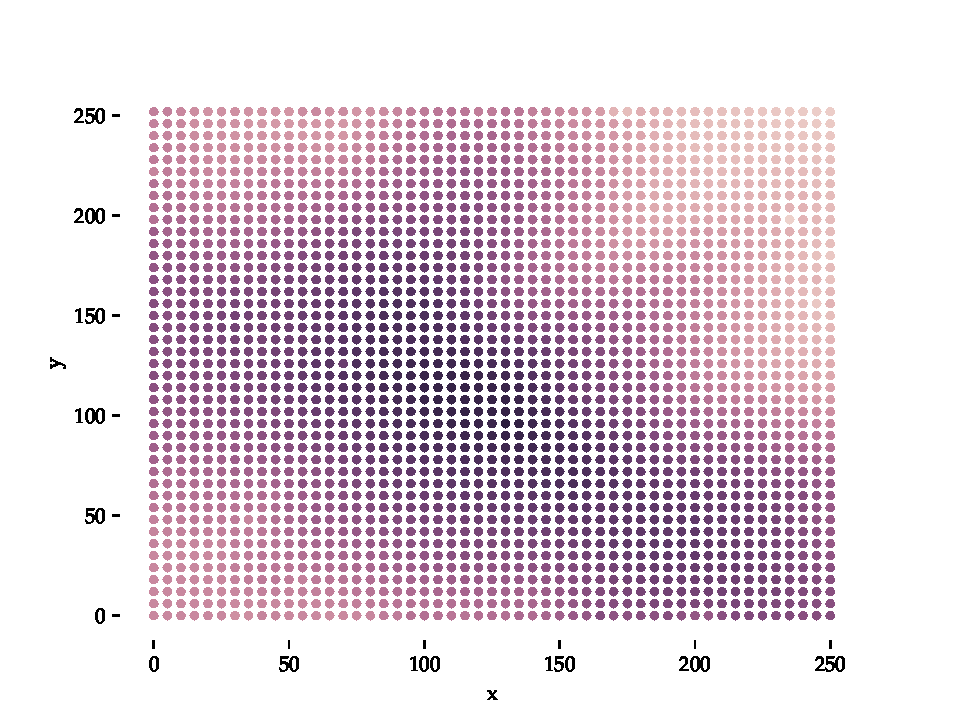
\includegraphics[width=0.5\linewidth]{figs/interpolation}
\caption{The result of using ordinary kriging to interpolate on a grid of points using the sample dataset using only the sample points within 15 units of each interpolated point.}%
\label{fig:interpolation}
\end{figure}

Finally, it is also important to consider some computational aspects into account.
If a large number of sample points are used to interpolate every point, ordinary kriging can be \emph{very slow}.
The reason for this is because matrix \(A\) will be very large, and inverting a matrix is a computationally expensive process.
However, inverting very large matrices is not really needed in practice.
When a sample point is far from the interpolated point, its weight will be low, and it will thus have a negligible influence on it.
Because of this, it is usually best to only take into account a few sample points in the calculation, either by limiting the sample points to those within a given search radius, or by selecting only a given number of its closest sample points.

% \section{Universal kriging}

%%%
%
\section{Notes and comments}

\citet{Krige51} is the original publication by Danie Krige, which was later formalised by Georges Matheron~\citep{Matheron62,Matheron65}.

A relatively simple explanation of Kriging with agricultural examples that is accessible from the campus or VPN is given by \citet{Oliver15}.
A standard reference textbook is \citet{Wackernagel03}.
 

%%%
%
\section{Exercises}

